\ifx\wholebook\relax \else
% ------------------------

\documentclass[b5paper]{ctexart}
\usepackage[nomarginpar
  %, margin=.5in
]{geometry}

\addtolength{\oddsidemargin}{-0.05in}
\addtolength{\evensidemargin}{-0.05in}
\addtolength{\textwidth}{0.1in}

\usepackage[cn]{../../../prelude}

\setcounter{page}{1}

\begin{document}

\title{AVL树}

\author{刘新宇
\thanks{{\bfseries 刘新宇} \newline
  Email: liuxinyu95@gmail.com \newline}
  }

\maketitle
\fi

\markboth{AVL树}{基本算法}

\ifx\wholebook\relax
\chapter{AVL树}
\numberwithin{Exercise}{chapter}
\fi

\label{introduction}
\index{AVL树}

为了解决平衡问题,红黑树限制在某一路径上的节点数。AVL树采用了更为直接方法:度量分枝间的差异。对于树$T$,定义:

\be
  \delta(T) = |r| - |l|
\ee

其中$|T|$表示树$T$的高度,$l$、$r$为左右子树。定义空树$\delta(\nil) = 0$。如果每棵子树$T$都有$\delta(T) = 0$,则树是完全平衡的。例如,一棵高度为$h$的完全二叉树有$n = 2^h - 1$个节点。除了叶子节点外,所有节点都不为空。$\delta(T)$的绝对值越小,树越平衡。我们称$\delta(T)$为二叉树的“平衡因子”。

\section{定义}
\index{AVL树!定义}

\begin{figure}[htbp]
   \centering
   \includegraphics[scale=0.5]{img/avl-example}
   \caption{AVL树} \label{fig:avl-example}
\end{figure}

一棵二叉搜索树称为AVL树,如果所有子树$T$都满足如下条件:

\be
  |\delta(T)| \leq 1
  \label{eq:avl-rule}
\ee

平衡因子$\delta(T)$只能是$\pm 1$、0。图\ref{fig:avl-example}给出了一棵AVL树的例子。如果树中有$n$个节点,这一定义保证了树的高度$h = O(\lg n)$。我们可以证明这个结论。一棵高为$h$的AVL树,其节点数目并不是一个固定的值。当它是完全二叉树时,含有的节点数目最多,为$2^h - 1$。我们关心它至少包含多少节点。定义$N(h)$代表高度为$h$的AVL树的最小节点数目。我们有:

\begin{itemize}
\item 空树$\nil$:$h = 0$,$N(0) = 0$;
\item 只有一个节点的树:$h = 1$,$N(1) = 1$;
\end{itemize}

图\ref{fig:N-h-relation}中给出了一个高度为$h$的AVL树$T$。它包含三部分:元素$k$和左右子树$l$、$r$。树的高度$h$和子树高度之间满足下面的关系:

\begin{figure}[htbp]
   \centering
   \includegraphics[scale=0.5]{img/Nh-lvr}
   \caption{高度为$h$的AVL树,其中一棵子树高$h - 1$,另外一棵的高度不小于$h - 2$}
   \label{fig:N-h-relation}
\end{figure}

\be
  h = max(|l|, |r|) + 1
\ee

因此必然存在一个子树的高度为$h - 1$。根据AVL树的定义,有 $||l| -|r|| \leq 1$。所以另外一棵子树的高度不会小于$h - 2$。而$T$所包含的节点数为两个子树的节点数和加1(节点$T$本身):

\be
  N(h) = N(h-1) + N(h-2) + 1
  \label{eq:Fibonacci-like}
\ee

这一递归形式让我们联想起斐波那契数列。如果定义$N'(h) = N(h) + 1$,我们就可以将(\ref{eq:Fibonacci-like})转换成斐波那契数列的递归关系:

\be
  N'(h) = N'(h-1) + N'(h-2)
\ee

\begin{lemma}
\label{lemma:N-phi}
若$N(h)$表示高为$h$的AVL树的节点数目最小值,令$N'(h) = N(h) + 1$,则:

\be
  N'(h) \geq \phi^h
\ee

其中$\phi = \dfrac{\sqrt{5}+1}{2}$,称为黄金分割比。
\end{lemma}

\begin{proof}[证明]
使用数学归纳法。当$h = 0$或1时:
\begin{itemize}
\item $h = 0$, $N'(0) = 1 \geq \phi^0 = 1$
\item $h = 1$, $N'(1) = 2 \geq \phi^1 = 1.618...$
\end{itemize}

对于递推情况,设$N'(h) \geq \phi^h$。
\[
  \begin{array}{lll}
  N'(h+1) & = N'(h) + N'(h-1) & \{Fibonacci\} \\
          & \geq \phi^h + \phi^{h-1} & \{\text{递推假设}\}\\
          & = \phi^{h-1}(\phi + 1) & \{\phi + 1 = \phi^2 = \dfrac{\sqrt{5}+3}{2}\} \\
          & = \phi^{h+1}
 \end{array}
\]
\end{proof}

由引理\ref{lemma:N-phi},我们立即得到下面的结果:

\be
  h \leq log_{\phi}(n+1) = log_{\phi}2 \cdot \lg (n+1) \approx 1.44 \lg (n+1)
  \label{eq:AVL-height}
\ee

这一不等式说明AVL树的高度为$O(\lg n)$,从而保证了平衡性。

插入和删除会改变树的结构,导致平衡因子的绝对值超出1,需要通过修复使得$|\delta| < 1$。传统的修复方法是树旋转。我们给出一种基于模式匹配的方法简化实现。思路类似于函数式的红黑树\cite{okasaki}。由于这种“改变——恢复”的策略,AVL树也是一种自平衡二叉树。我们复用二叉搜索树的定义,尽管平衡因子$\delta$可以递归地求出,为了方便,我们在每个非空节点$T = (l, k, r, \delta)$中保存平衡因子的值,并在改变树结构时更新它\footnote{也可以保存树的高度而非$\delta$\cite{py-avl}。}。下面的例子程序增加了一个整型变量$\delta$:

\lstset{frame = single}
\begin{Haskell}
data AVLTree a = Empty
               | Br (AVLTree a) a (AVLTree a) Int
\end{Haskell}

AVL树的$lookup$、$max$、$min$等操作和二叉搜索树相同,而插入和删除操作是特殊的。

\section{插入}
\index{AVL树!插入}

向AVL树中插入一个新元素时,平衡因子的绝对值$|\delta(T)|$可能超过1。我们用类似红黑树修复的模式匹配方法恢复平衡。插入元素$x$后,包含它的子树高度最多增加1。我们需要沿着插入路径递归地更新平衡因子。定义插入结果为一对值$(T', \Delta H)$,其中$T'$为插入后的树,$\Delta H$为高度的增加值。我们将二叉搜索树的插入算法修改如下:

\be
insert = \textit{fst} \circ ins
\ee

其中$\textit{fst}\ (a, b) = a$返回一对值中的第一个。$ins(T, k)$将元素$x$插入到树$T$中:

\be
\begin{array}{rcl}
ins\ \nil\ k & = & ((\nil, k, \nil, 0), 1) \\
ins\ (l, k', r, \delta)\ k & = & \begin{cases}
  k < k': tree\ (ins\ l\ k)\ k'\ (r, 0)\ \delta \\
  k > k': tree\ (l, 0)\ k'\ (ins\ r, k)\ \delta \\
\end{cases}
\end{array}
\label{eq:ins}
\ee

如果树为空$\nil$,结果为包含$k$的叶子节点,平衡因子为0,高度增加1。否则,令$T = (l, k', r, \delta)$。我们比较$k$和$k'$,如果$k < k'$,我们递归地将$k$插入到左子树$l$中,否则插入右子树$r$。递归插入的结果也是一对值$(l', \Delta l)$或$(r', \Delta r)$。我们通过函数$tree$调整平衡因子并更新高度,它接受4个参数:$(l', \Delta l)$、$k'$、$(r', \Delta r)$、$\delta$,并产生结果$(T', \Delta H)$。其中$T'$为新树,$\Delta H$定义如下:

\be
  \Delta H = |T'| - |T|
\ee

它可以进一步分解为4种情况:

\be
\begin{array}{rcl}
  \Delta H & = & |T'| - |T| \\
           & = & 1 + max(|r'|, |l'|) - (1 + max(|r|, |l|)) \\
           & = & max(|r'|, |l'|) - max(|r|, |l|) \\
           & = & \begin{cases}
\delta \geq 0, \delta' \geq 0: & \Delta r \\
\delta \leq 0, \delta' \geq 0: & \delta + \Delta r \\
\delta \geq 0, \delta' \leq 0: & \Delta l - \delta \\
\text{否则}: & \Delta l
\end{cases}
\end{array}
\ee

其中$\delta' = \delta(T') = |r'| - |l'|$,是变化后的平衡因子。附录B给出了相关证明。在平衡调整前,还需要确定新的平衡因子$\delta'$。

\be
\begin{array}{rcl}
\delta' & = & |r'| - |l'| \\
        & = & |r| + \Delta r - (|l| + \Delta l) \\
        & = & |r| - |l| + \Delta r - \Delta l \\
        & = & \delta + \Delta r - \Delta l \\
\end{array}
\ee

使用树的高度变化和平衡因子,就可进一步定义(\ref{eq:ins})中的函数$tree$:

\be
tree\ (l', \Delta l)\ k\ (r', \Delta r)\ \delta =
  balance\ (l', k, r', \delta')\ \Delta H
\ee

下面的例子程序实现了目前给出的结论:

\begin{Haskell}
insert t x = fst $ ins t where
    ins Empty = (Br Empty x Empty 0, 1)
    ins (Br l k r d)
        | x < k = tree (ins l) k (r,  0) d
        | x > k = tree (l,  0) k (ins r) d

tree (l, dl) k (r, dr) d = balance (Br l k r d') deltaH where
    d' = d + dr - dl
    deltaH | d >=0 && d' >=0 = dr
           | d <=0 && d' >=0 = d+dr
           | d >=0 && d' <=0 = dl - d
           | otherwise = dl
\end{Haskell} %$

\subsection{平衡调整}
\index{AVL树!平衡调整}
共有4种情况需要修复,如图\ref{fig:avl-insert-fix}所示。平衡因子为$\pm 2$超出了$[-1, 1]$范围。我们将其统一调整为图中心的结构,使得$\delta(y) = 0$。

\begin{figure}[htbp]
  \centering
  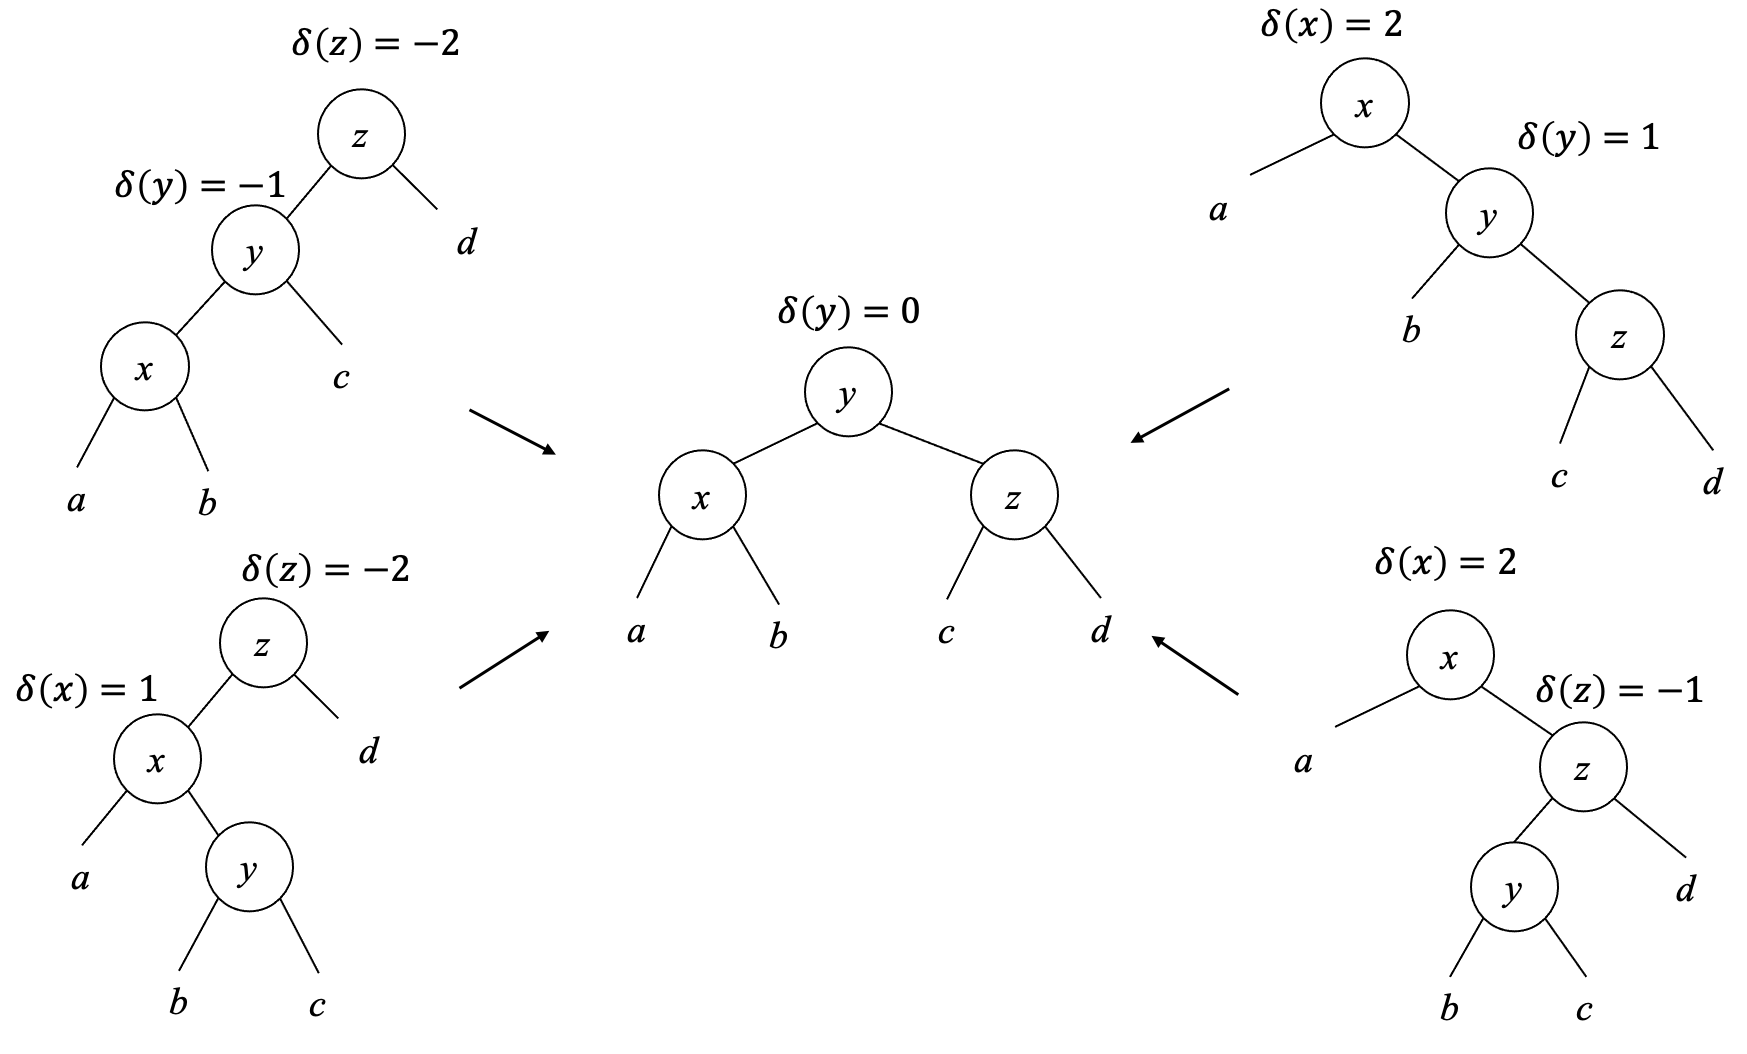
\includegraphics[scale=0.4]{img/avl-insert-fix}
  \caption{将4种情况修复为统一形式}
  \label{fig:avl-insert-fix}
\end{figure}

我们称这4种情况为左-左、右-右、右-左、左-右。记调整前的平衡因子为$\delta(x)$、$\delta(y)$、$\delta(z)$;调整后的平衡因子为$\delta'(x)$、$\delta'(y) = 0$、$\delta'(z)$。它们的关系如下。附录B给出了证明。

左-左:

\be
  \begin{array}{l}
  \delta'(x) = \delta(x) \\
  \delta'(y) = 0 \\
  \delta'(z) = 0
  \end{array}
\ee

右-右:

\be
  \begin{array}{l}
  \delta'(x) = 0 \\
  \delta'(y) = 0 \\
  \delta'(z) = \delta(z)
  \end{array}
  \label{eq:rr-result}
\ee

右-左和左-右:

\be
  \begin{array}{l}
  \delta'(x) = \begin{cases}
    \delta(y) = 1: & -1 \\
    otherwise: & 0 \\
    \end{cases} \\
  \delta'(y) = 0 \\
  \delta'(z) = \begin{cases}
    \delta(y) = -1: & 1 \\
    otherwise: & 0 \\
    \end{cases} \\
  \end{array}
  \label{eq:rl-result}
\ee

利用模式匹配,可将修复定义如下:

\be
\resizebox{\textwidth}{!}{\ensuremath{
\begin{array}{rcl}
balance\ (((a, x, b, \delta(x)), y, c, -1), z, d, -2)\ \Delta H & = & ((a, x, b, \delta(x)), y, (c, z, d, 0), 0, \Delta H -1) \\
balance\ (a, x, (b, y, (c, z, d, \delta(z)), 1), 2)\ \Delta H & = & ((a, x, b, 0), y, (c, z, d, \delta(z)), 0, \Delta H -1) \\
balance\ ((a, x, (b, y, c, \delta(y)), 1), z, d, -2)\ \Delta H & = & ((a, x, b, \delta'(x)), y, (c, z, d, \delta'(z)), 0, \Delta H - 1) \\
balance\ (a, x, ((b, y, c, \delta(y)), z, d, -1), 2)\ \Delta H & = & ((a, x, b, \delta'(x)), y, (c, z, d, \delta'(z)), 0, \Delta H - 1) \\
balance\ T\ \Delta H & = & (T, \Delta H) \\
\end{array}
}}
\ee

其中$\delta'(x)$和$\delta'(z)$按照式(\ref{eq:rl-result})定义。如果没有匹配任何模式,最后一行保持树不变。下面是相应的例子程序:

\begin{Haskell}
balance (Br (Br (Br a x b dx) y c (-1)) z d (-2)) dH =
            (Br (Br a x b dx) y (Br c z d 0) 0, dH-1)
balance (Br a x (Br b y (Br c z d dz)    1)    2) dH =
            (Br (Br a x b 0) y (Br c z d dz) 0, dH-1)
balance (Br (Br a x (Br b y c dy)    1) z d (-2)) dH =
            (Br (Br a x b dx') y (Br c z d dz') 0, dH-1) where
    dx' = if dy ==  1 then -1 else 0
    dz' = if dy == -1 then  1 else 0
balance (Br a x (Br (Br b y c dy) z d (-1))    2) dH =
            (Br (Br a x b dx') y (Br c z d dz') 0, dH-1) where
    dx' = if dy ==  1 then -1 else 0
    dz' = if dy == -1 then  1 else 0
balance t d = (t, d)
\end{Haskell}

插入算法的复杂度和树的高度成正比,根据式(\ref{eq:AVL-height}),对于$n$个节点的树,$insert$的复杂度为$O(\lg n)$。

\subsubsection{验证}
\index{AVL树!验证}

为了验证AVL树,我们需要检查两点:是否是二叉搜索树;对于每棵子树$T$,式(\ref{eq:avl-rule}):$\delta(T) \leq 1$是否成立。下面的函数递归地检查子树间的高度差:

\be
\begin{array}{rcl}
avl?\ \nil & = & \textit{True} \\
avl?\ T & = & avl?\ l\ \land avl?\ r\ \land ||r| - |l|| \leq 1 \\
\end{array}
\ee

其中$l$、$r$分别是左右子树,高度递归计算如下:

\be
\begin{array}{rcl}
|\nil| & = & 0 \\
|T| & = & 1 + max(|r|, |l|) \\
\end{array}
\ee

下面的例子程序实现了AVL树高度的检查:
\begin{Haskell}
isAVL Empty = True
isAVL (Br l _ r _) = isAVL l && isAVL r && abs (height r - height l) <= 1

height Empty = 0
height (Br l _ r _) = 1 + max (height l) (height r)
\end{Haskell}

\begin{Exercise}
\Question{我们只验证了AVL树的高度性质,完成验证程序检查一棵二叉树是否是AVL树。}
\end{Exercise}

\section{AVL树的命令式算法$\bigstar$}
\index{AVL树!命令式插入}

为了完整,本节给出AVL树的命令式算法。和红黑树的命令式算法相似,我们先按二叉搜索树将新元素插入,然后再通过旋转操作恢复平衡。

\begin{algorithmic}[1]
\Function{Insert}{$T, k$}
  \State $root \gets T$
  \State $x \gets$ \Call{Create-Leaf}{$k$}
  \State \Call{$\delta$}{$x$} $\gets 0$
  \State $parent \gets$ NIL
  \While{$T \neq$ NIL}
    \State $parent \gets T$
    \If{$k <$ \Call{Key}{$T$}}
      \State $T \gets $ \Call{Left}{$T$}
    \Else
      \State $T \gets $ \Call{Right}{$T$}
    \EndIf
  \EndWhile
  \State \Call{Parent}{$x$} $\gets parent$
  \If{$parent =$ NIL} \Comment{树$T$为空}
    \State \Return $x$
  \ElsIf{$k <$ \Call{Key}{$parent$}}
    \State \Call{Left}{$parent$} $\gets x$
  \Else
    \State \Call{Right}{$parent$} $\gets x$
  \EndIf
  \State \Return \Call{AVL-Insert-Fix}{$root, x$}
\EndFunction
\end{algorithmic}

插入新元素后,树的高度可能增加,因此平衡因子$\delta$也会变化。插入到右侧可能使$\delta$增加1,插入左侧可能使$\delta$减少1。我们从$x$开始,自底向上修复平衡,直到根节点。记新的平衡因子为$\delta'$,共有3种情况:

\begin{itemize}
\item $|\delta| = 1$、$|\delta'| = 0$。插入后树处于平衡状态。父节点的高度没有变化。

\item $|\delta| = 0$、$|\delta'| = 1$。左右子树之一的高度增加了,需要继续向上检查平衡。

\item $|\delta| = 1$、$|\delta'| = 2$。需要旋转以修复平衡。
\end{itemize}

\begin{algorithmic}[1]
\Function{AVL-Insert-Fix}{$T, x$}
  \While{\Call{Parent}{$x$} $\neq$ NIL}
    \State $\delta \gets $ \textproc{$\delta$}(\Call{Parent}{$x$})
    \If{$x = $ \textproc{Left}(\Call{Parent}{$x$})}
      \State $\delta' \gets \delta - 1$
    \Else
      \State $\delta' \gets \delta + 1$
    \EndIf
    \State \textproc{$\delta$}(\Call{Parent}{$x$}) $\gets \delta'$
    \State $P \gets $ \Call{Parent}{$x$}
    \State $L \gets $ \Call{Left}{$x$}
    \State $R \gets $ \Call{Right}{$x$}
    \If{$|\delta| = 1$ and $|\delta'| = 0$} \Comment{高度没有变化}
      \State \Return $T$
    \ElsIf{$|\delta| = 0$ and $|\delta'| = 1$} \Comment{继续自底向上更新}
      \State $x \gets P$
    \ElsIf{$|\delta| = 1$ and $|\delta'| = 2$}
      \If{$\delta'=2$}
        \If{$\delta(R) = 1$} \Comment{右-右}
          \State $\delta(P) \gets 0$ \Comment{根据式(\ref{eq:rr-result})}
          \State $\delta(R) \gets 0$
          \State $T \gets $ \Call{Left-Rotate}{$T, P$}
        \EndIf
        \If{$\delta(R) = -1$} \Comment{右-左}
          \State $\delta_y \gets $ \textproc{$\delta$}(\Call{Left}{$R$}) \Comment{根据式(\ref{eq:rl-result})}
          \If{$\delta_y = 1$}
            \State $\delta(P) \gets -1$
          \Else
            \State $\delta(P) \gets 0$
          \EndIf
          \State \textproc{$\delta$}(\Call{Left}{$R$}) $\gets 0$
          \If{$\delta_y = -1$}
            \State $\delta(R) \gets 1$
          \Else
            \State $\delta(R) \gets 0$
          \EndIf
          \State $T \gets $ \Call{Right-Rotate}{$T, R$}
          \State $T \gets $ \Call{Left-Rotate}{$T, P$}
        \EndIf
      \EndIf
      \If{$\delta' = -2$}
        \If{$\delta(L) = -1$} \Comment{左-左}
          \State $\delta(P) \gets 0$
          \State $\delta(L) \gets 0$
          \State \Call{Right-Rotate}{$T, P$}
        \Else \Comment{左-右}
          \State $\delta_y \gets $ \textproc{$\delta$}(\Call{Right}{$L$})
          \If{$\delta_y = 1$}
            \State $\delta(L) \gets -1$
          \Else
            \State $\delta(L) \gets 0$
          \EndIf
          \State \textproc{$\delta$}(\Call{Right}{$L$}) $\gets 0$
          \If{$\delta_y = -1$}
            \State $\delta(P) \gets 1$
          \Else
            \State $\delta(P) \gets 0$
          \EndIf
          \State \Call{Left-Rotate}{$T, L$}
          \State \Call{Right-Rotate}{$T, P$}
        \EndIf
      \EndIf
      \State break
    \EndIf
  \EndWhile
  \State \Return $T$
\EndFunction
\end{algorithmic}

除了旋转,还需要更新平衡因子$\delta$。右-右和左-左情况需要进行一次旋转;而右-左和左-右需要进行两次旋转。我们略过了AVL树的删除算法,附录B给出了删除的实现。

\section{小结}
AVL树是1962年由Adelson-Velskii和Landis\cite{wiki-avl}、\cite{TFATP}提出的,并以两位作者的名字命名。它比红黑树更早。AVL树和红黑树都是自平衡二叉搜索树,大多数操作的复杂度都是$O(\lg n)$。式(\ref{eq:AVL-height})使得AVL树的平衡性更为严格。在大量查询的情况下,其表现要好于红黑树\cite{wiki-avl}。但红黑树在频繁插入和删除的情况下性能更佳。很多程序库使用红黑树作为自平衡二叉搜索树的内部实现,AVL树同样也可以直观、高效地解决平衡问题。

\section{附录:例子程序}

AVL树的定义:

\begin{lstlisting}[language = Bourbaki]
data Node<T> {
    int delta
    T key
    Node<T> left
    Node<T> right
    Node<T> parent
}
\end{lstlisting}

平衡修复:

\begin{lstlisting}[language = Bourbaki]
Node<T> insertFix(Node<T> t, Node<T> x) {
    while (x.parent != null ) {
        var (p, l, r) = (x.parent, x.parent.left, x.parent.right)
        var d1 = p.delta
        var d2 = if x == parent.left then d1 - 1 else d1 + 1
        p.delta = d2

        if abs(d1) == 1 and abs(d2) == 0 {
            return t
        } else if abs(d1) == 0 and abs(d2) == 1 {
            x = p
        } else if abs(d1) == 1 and abs(d2) == 2 {
            if d2 == 2 {
                if r.delta == 1 {    //Right-right
                    p.delta = 0
                    r.delta = 0
                    t = rotateLeft(t, p)
                } else if r.delta == -1 {    //Right-Left
                    var dy = r.left.delta
                    p.delta = if dy == 1 then -1 else 0
                    r.left.delta = 0
                    r.delta = if dy == -1 then 1 else 0
                    t = rotateRight(t, r)
                    t = rotateLeft(t, p)
                }
            } else if d2 == -2 {
                if l.delta == -1 {    //Left-left
                    p.delta = 0
                    l.delta = 0
                    t = rotateRight(t, p)
                } else if l.delta == 1 {    //Left-right
                    var dy = l.right.delta
                    l.delta = if dy == 1 then -1 else 0
                    l.right.delta = 0
                    p.delta = if dy == -1 then 1 else 0
                    t = rotateLeft(t, l)
                    t = rotateRight(t, p)
                }
            }
            break
        }
    }
    return t
}
\end{lstlisting}

\ifx\wholebook\relax \else
\begin{thebibliography}{99}

\bibitem{hackage-avl}
Data.Tree.AVL \url{http://hackage.haskell.org/packages/archive/AvlTree/4.2/doc/html/Data-Tree-AVL.html}

\bibitem{okasaki}
Chris Okasaki. ``FUNCTIONAL PEARLS Red-Black Trees in a Functional Setting''. J. Functional Programming. 1998

\bibitem{wiki-avl}
Wikipedia. ``AVL tree''. \url{https://en.wikipedia.org/wiki/AVL_tree}

\bibitem{TFATP}
Guy Cousinear, Michel Mauny. ``The Functional Approach to Programming''. Cambridge University Press; English Ed edition (October 29, 1998). ISBN-13: 978-0521576819

\bibitem{py-avl}
Pavel Grafov. ``Implementation of an AVL tree in Python''. \url{http://github.com/pgrafov/python-avl-tree}
\end{thebibliography}

\end{document}
\fi

% LocalWords:  AVL Okasaki STL
